\subsection{DHCP and static IP}
To analyse the power consumption when connecting via DHCP or with a static IP, we monitored the current of an average connection process.\\

\subsubsection{Experimental setup}
The sequence of the test program for DHCP is the same as Fig. \ref{fig:experiment_deep_sleep} shows.
Fig. \ref{fig:experiment_static_ip} shows the sequence when conducting the experiment using a static IP address.
The ESP8266-01 WiFi library provides functionality to set a static IP address.\\

\subsubsection{DHCP}
As shown in Fig. \ref{fig:dhcp}, the establishment of the connection to the network by using DHCP takes $\approx 5.5 s$.
In average, the average current consumption is $\approx 68.9 mA$ and in total, it consumes about $0.3545 As\ (\sigma = 0.00065$) as seen in Fig. \ref{fig:dhcp_boxplot}.
It is mentionable that in this case, everytime the device connects to the network, it gets a new IP address.
This happens because the lease time runs out before the device reconnects again.
This can be optimized by setting longer lease times.
When the lease time is long enough and the device doesn't get a new IP address, it takes around the same energy as using a static IP address.\\

\subsubsection{Static IP address}
In Fig. \ref{fig:static_ip} a connection cycle to the WiFi network by using a static IP address is shown.
The connection to the WiFi network by using a static IP address takes $\approx 4 s$.
The average current consumption is $\approx 68.9 mA$.
As the establishment of the connection takes less time, it consumes about $0.2821 A\ (\sigma = 0.00085)$  in total, as seen in Fig. \ref{fig:static_boxplot}.
The duration of the establishment of the connection is shorter, because there is no commnucation with the DHCP server needed.


\begin{figure}[h]
    \centering
    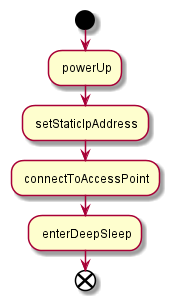
\includegraphics[width = 0.35 \linewidth]{fig/sequence_static_ip.png}
    \caption{Experimental setup for use of a static IP.}
    \label{fig:experiment_static_ip}
\end{figure}
\begin{figure}[h]
    \centering
    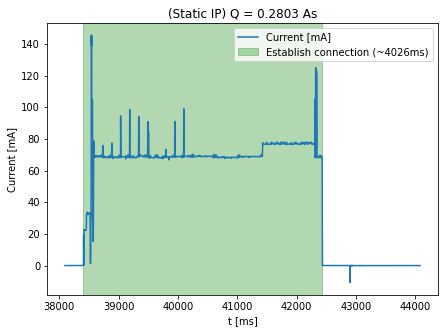
\includegraphics[width =\linewidth]{fig/static_ip.png}
    \caption{Experimental setup for use of a static IP.}
    \label{fig:static_ip}
\end{figure}
\begin{figure}[h]
    \centering
    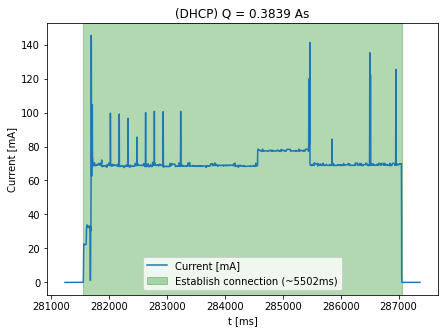
\includegraphics[width =\linewidth]{fig/dhcp.png}
    \caption{Experimental setup for use of DHCP with new IP address every reconnect.}
    \label{fig:dhcp}
\end{figure}
\begin{figure}[h]
    \centering
    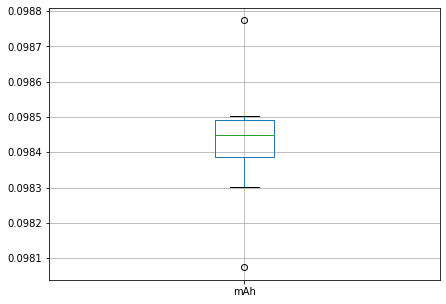
\includegraphics[width =\linewidth]{fig/dhcp_boxplot.png}
    \caption{$As$ of one connection interval with DHCP.}
    \label{fig:dhcp_boxplot}
\end{figure}
\begin{figure}[h]
    \centering
    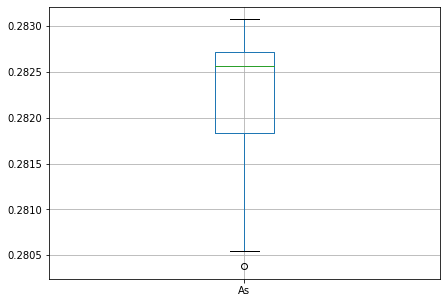
\includegraphics[width =\linewidth]{fig/static_boxplot.png}
    \caption{$As$ of one connection interval with Static IP.}
    \label{fig:static_boxplot}
\end{figure}
\pagebreak